\documentclass[english, xcolor={table}]{beamer}
\usepackage{graphicx}
\usepackage[english]{babel}
\usepackage[utf8]{inputenx}
\usepackage[T1]{fontenc}      % Font encoding
\usepackage{palatino}          % lmodern font, correctly copyable characters in pdf
\usepackage{hyperref}         % Hyperlinks
\usepackage{amsmath}          % Math
\usepackage{amssymb}          % Math symbols
\usepackage{mathtools}        % Math tools
\usepackage{microtype}        % Microtypography
\usepackage{csquotes}
\usepackage{bookmark}
\usepackage{subfigure}
\usepackage{tikz}
\usepackage{chngcntr}
\usepackage{ragged2e}
\counterwithin{subfigure}{figure}
\usepackage{caption}
\usepackage{listings}
\usepackage{tabularx}
\usepackage{booktabs}         % Tables
\usepackage{float}
\usepackage{listings}
\usepackage{bera}
\usepackage{cleveref}

%%%% COMPILE WITH LATEXMK %%%%

\usetheme[
  bullet=circle,                  % Use circles instead of squares for bullets
  titleline=false,                % Show a line below the frame
  alternativetitlepage=true,      % Use the fancy title
  titlepagelogo=logo-sapienza,    % Logo for the first slide
  watermark=watermark-diag,       % Watermark used in every slide
  watermarkheight=20px,           % Desired height of the watermark
  watermarkheightmult=6,          % Watermark image is actually x times bigger
  displayauthoronfooter=true,     % Display author name in the footer
]{Roma}
\watermarkoff%
\author{\scriptsize \textbf{Dario Loi}  \textbf{(1940849)}  \\ \textbf{Alessandro Monteleone} \textbf{(1883922)}}

\title{Advanced Machine Learning}
\subtitle{Final Project Presentation --- MobileViTs for Sign Language Recognition}
\institute{M.Sc. in Computer Science, \\ Sapienza, University of Rome.}
\date{A. Y. 2024 -- 2025}

% Cover future items, do not cover past items

\setbeamercovered{transparent=20}

\colorlet{punct}{red!60!black}
\definecolor{background}{HTML}{EEEEEE}
\definecolor{delim}{RGB}{20,105,176}
\colorlet{numb}{magenta!60!black}

% BiBTeX

\begin{document}

\maketitle

\section{Task and Motivation}

\begin{frame}
  \frametitle{Task and Motivation}

  \begin{columns}
    \begin{column}{0.5\textwidth}
        \textbf{Task:} Continuous Sign Language Recognition (CSLR).
        A \alert{sequence-to-sequence} problem, where the input is a video and the output is a phrase in natural language.
    \end{column}
    \begin{column}{0.5\textwidth}
        \textbf{Dataset:} RWTH-PHOENIX-Weather 2014T.
        Around $\approx 4$ thousand videos, $25$ frames per second, $210 \times 260$ pixels.
      \end{column}
  \end{columns}
\end{frame}

\section{MobileViTs}

\begin{frame}
  \frametitle{MobileViTs}

  \begin{columns}
    \begin{column}{0.3\textwidth}
      \alert{MobileViTs}\cite{mehta_mobilevit_2022} are a lightweight version of Vision Transformers (ViTs) that are designed to run on \alert{mobile devices}.
    \end{column}
    \begin{column}{0.7\textwidth}
      \begin{figure}
        \centering
        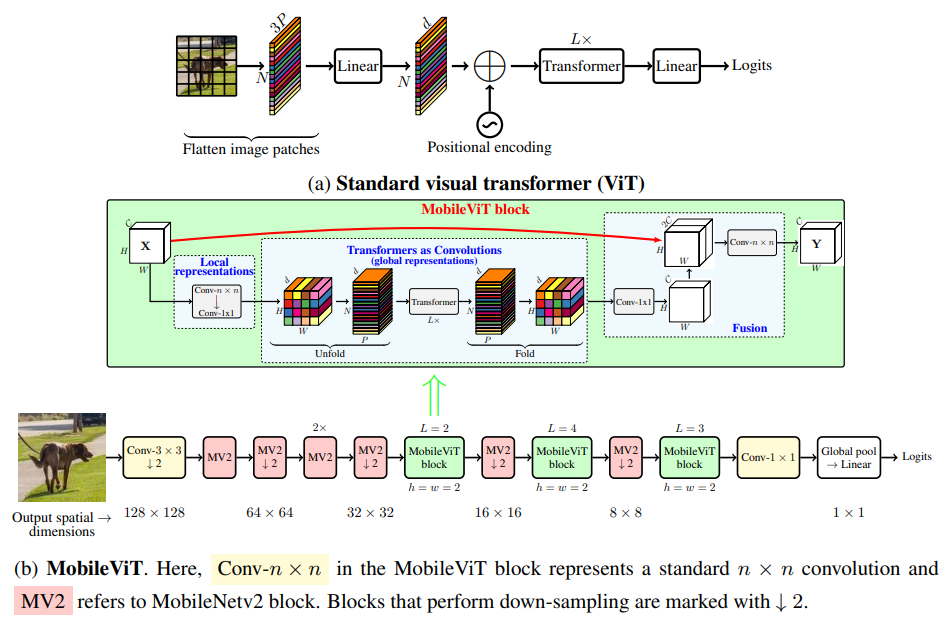
\includegraphics[width=1\textwidth]{figures/arch.png}
        \caption{MobileViT architecture.}
      \end{figure}
    \end{column}
  \end{columns}
\end{frame}

\begin{frame}
  \frametitle{Our novel MobileViT architecture}

  \begin{columns}
    \begin{column}{0.6\textwidth}
      We adapt the MobileViT architecture to CSLR by performing \alert{spatio-temporal} aggregation across \alert{multiple frames}. 
      This comes at no additional cost in terms of parameters, while allowing full exploitation of the temporal dimension.
    \end{column}
    \begin{column}{0.4\textwidth}
      \begin{figure}
        \centering
        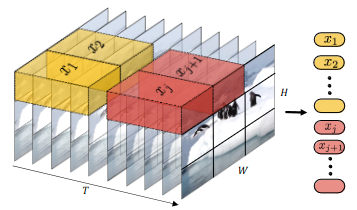
\includegraphics[width=1\textwidth]{figures/tubelet.png}
        \caption{When the temporal dimension is processed in patches, the volume is called a \alert{tubelet}.}
      \end{figure}
    \end{column}
  \end{columns}
\end{frame}

\section{Approaches}

\begin{frame}
  \frametitle{First approach: Encoder-only MobileViT}

  \begin{columns}
    \begin{column}{0.6\textwidth}
      To ensure a \alert{minimal} amount of parameters, we first tried to train an encoder-only MobileViT. We use \alert{CTC loss} to perform per-frame prediction of tokens from the encoder output, fusing repeated tokens.
    \end{column}
    \begin{column}{0.4\textwidth}
      \begin{figure}
        \centering
        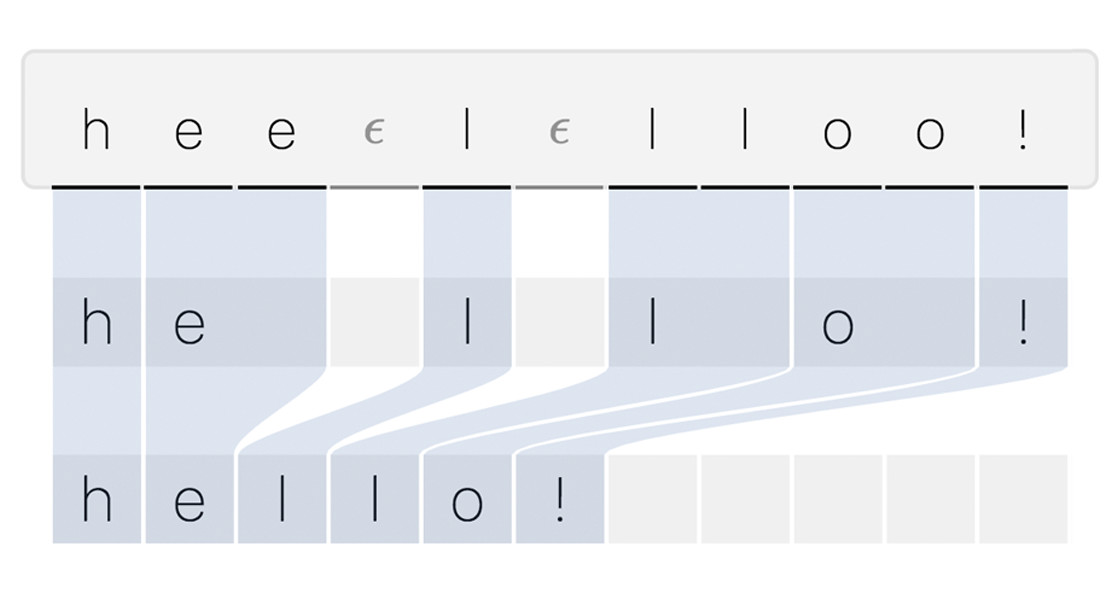
\includegraphics[width=1\textwidth]{figures/ctc_decoding.jpg}
        \caption{Output of a CTC loss trained model. repeated tokens separated by a blank token are fused.}
      \end{figure}
    \end{column}
  \end{columns}
\end{frame}

\begin{frame}
  \frametitle{Second approach: Encoder-decoder MobileViT}

    To compare ourselves with a more classical approach, we also trained an \alert{encoder-decoder} MobileViT. We attach a decoder head to the encoder output, and train the model with classic CE loss and teacher forcing.

    This \alert{massively} increases the number of parameters w.r.t. the encoder-only model, but it \alert{simplifies} the training process.

\end{frame}

\section{Experiments \& Results}

\begin{frame}
  \frametitle{Encoder-only MobileViT: Results}

  The encoder-only model gets trapped in a local minimum (predicting 0-length sequences) and does not recover. Repeated experiments with different configurations did \alert{not} yield better results.

  \begin{columns}
    \begin{column}{0.5\textwidth}
      \begin{figure}
        \centering
        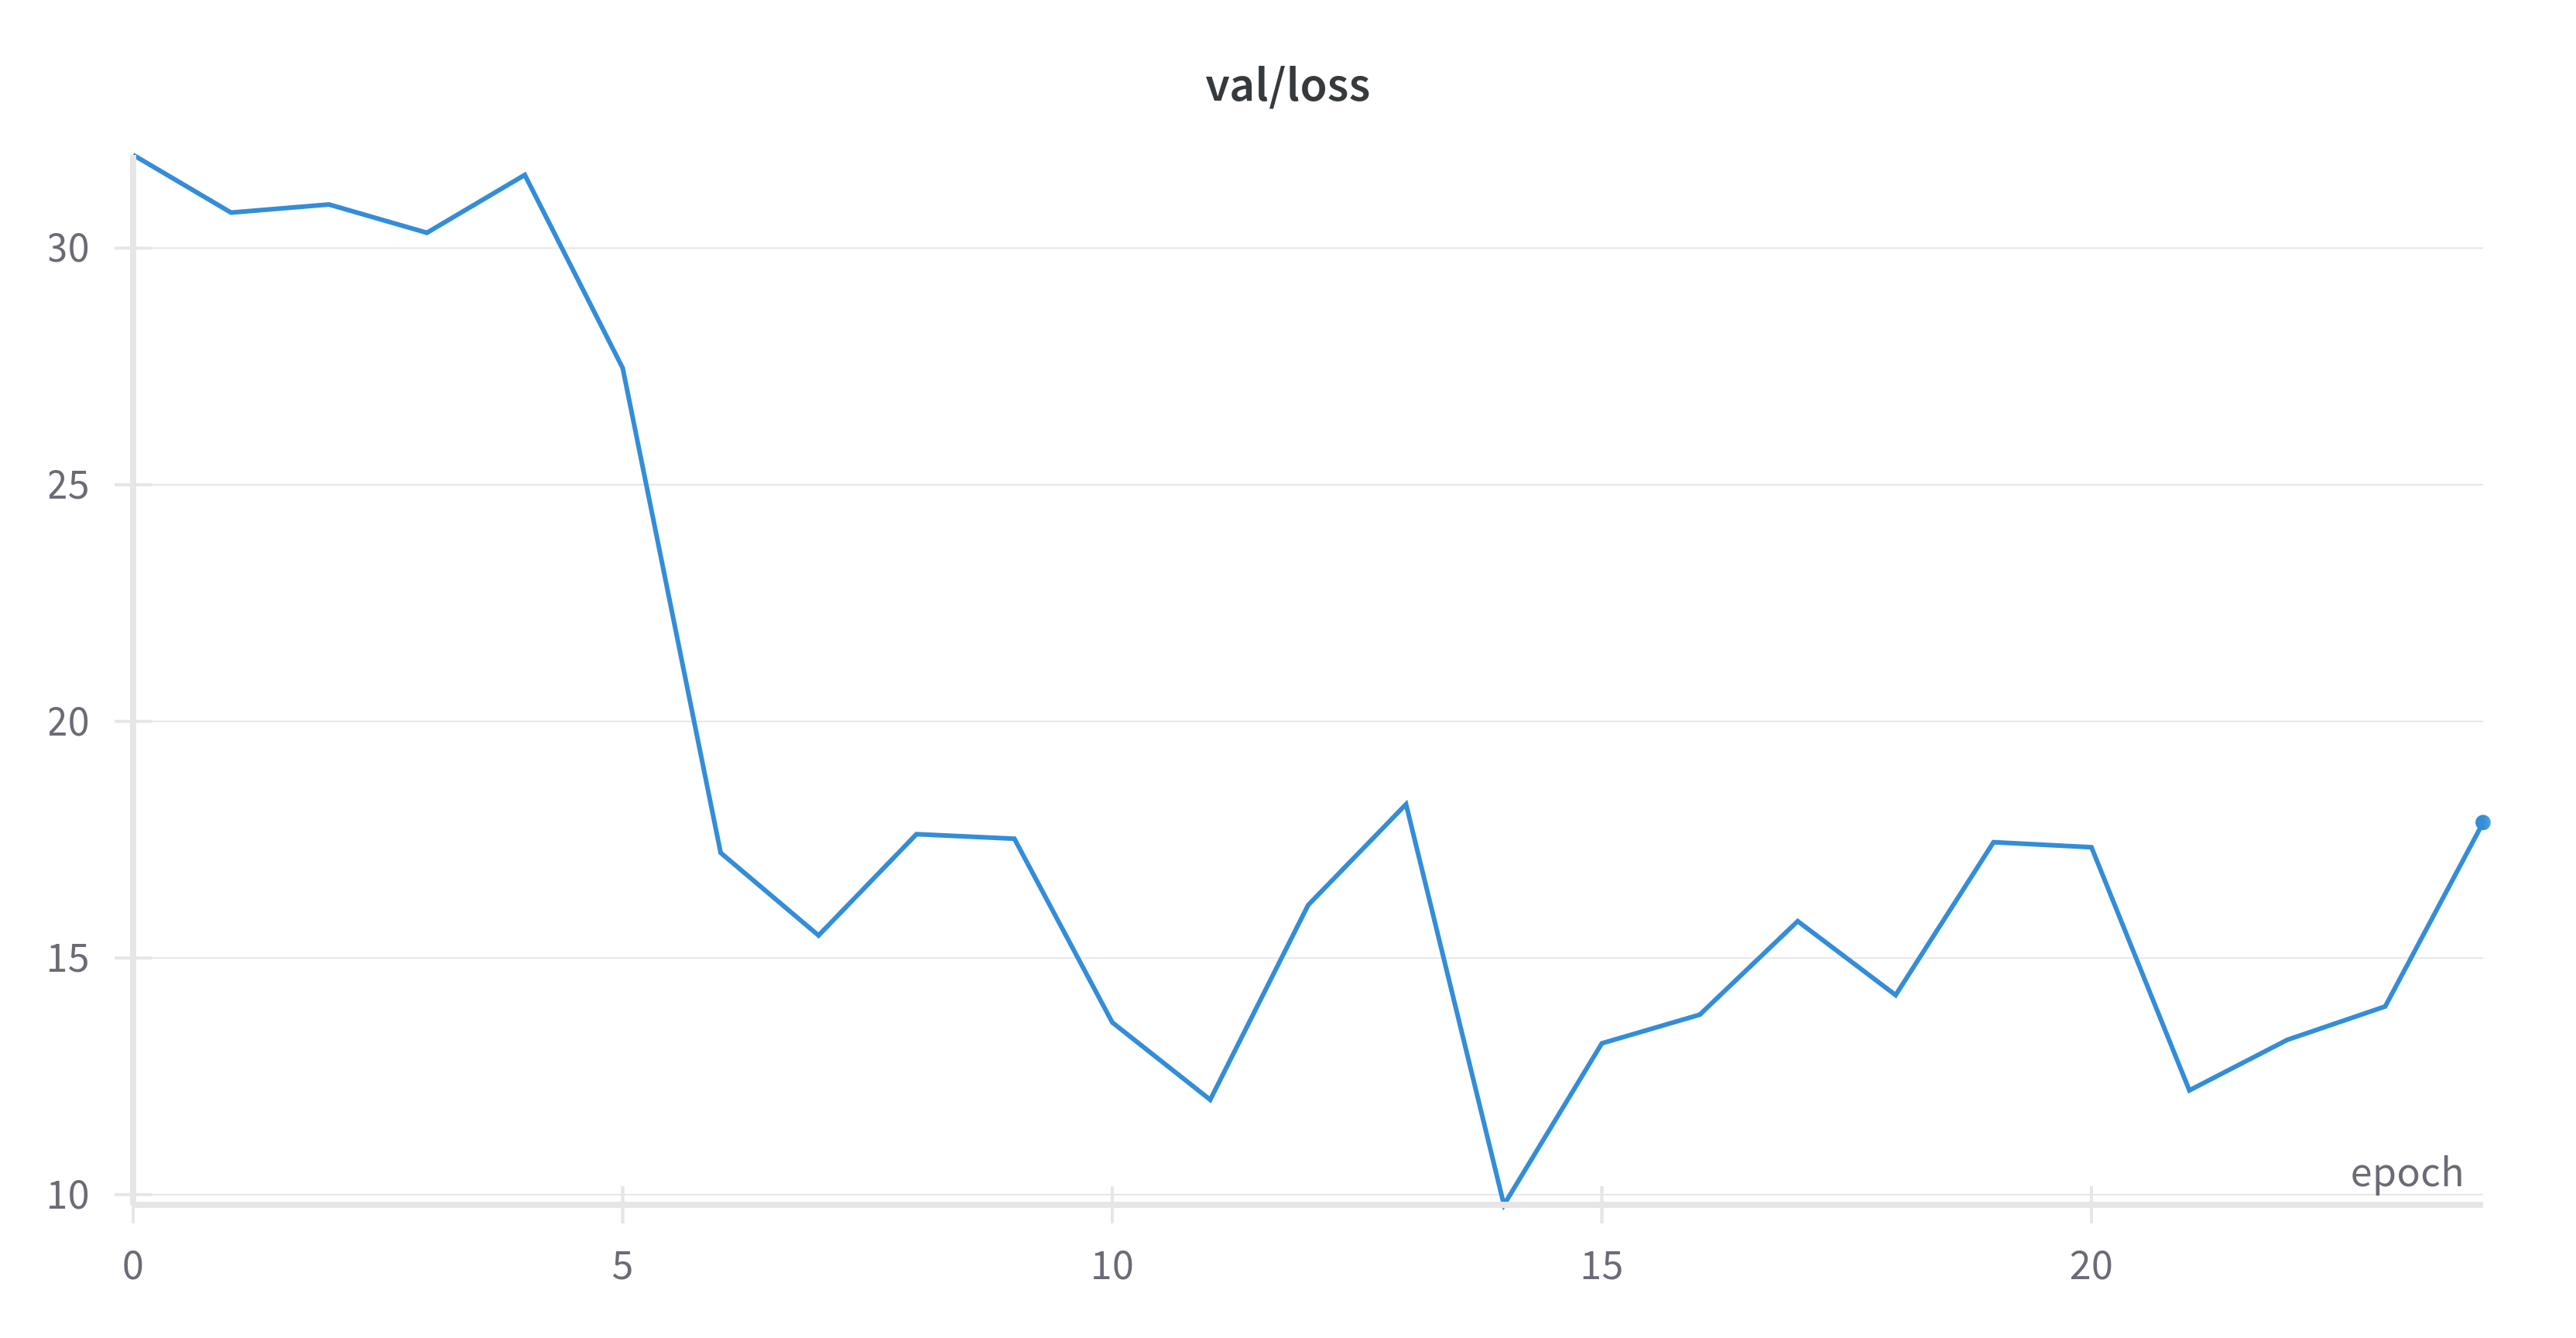
\includegraphics[width=1\textwidth]{figures/loss_ctc.png}
        \caption{Validation loss for the encoder-only MobileViT.}
      \end{figure}
    \end{column}
    \begin{column}{0.5\textwidth}
      \begin{figure}
        \centering
        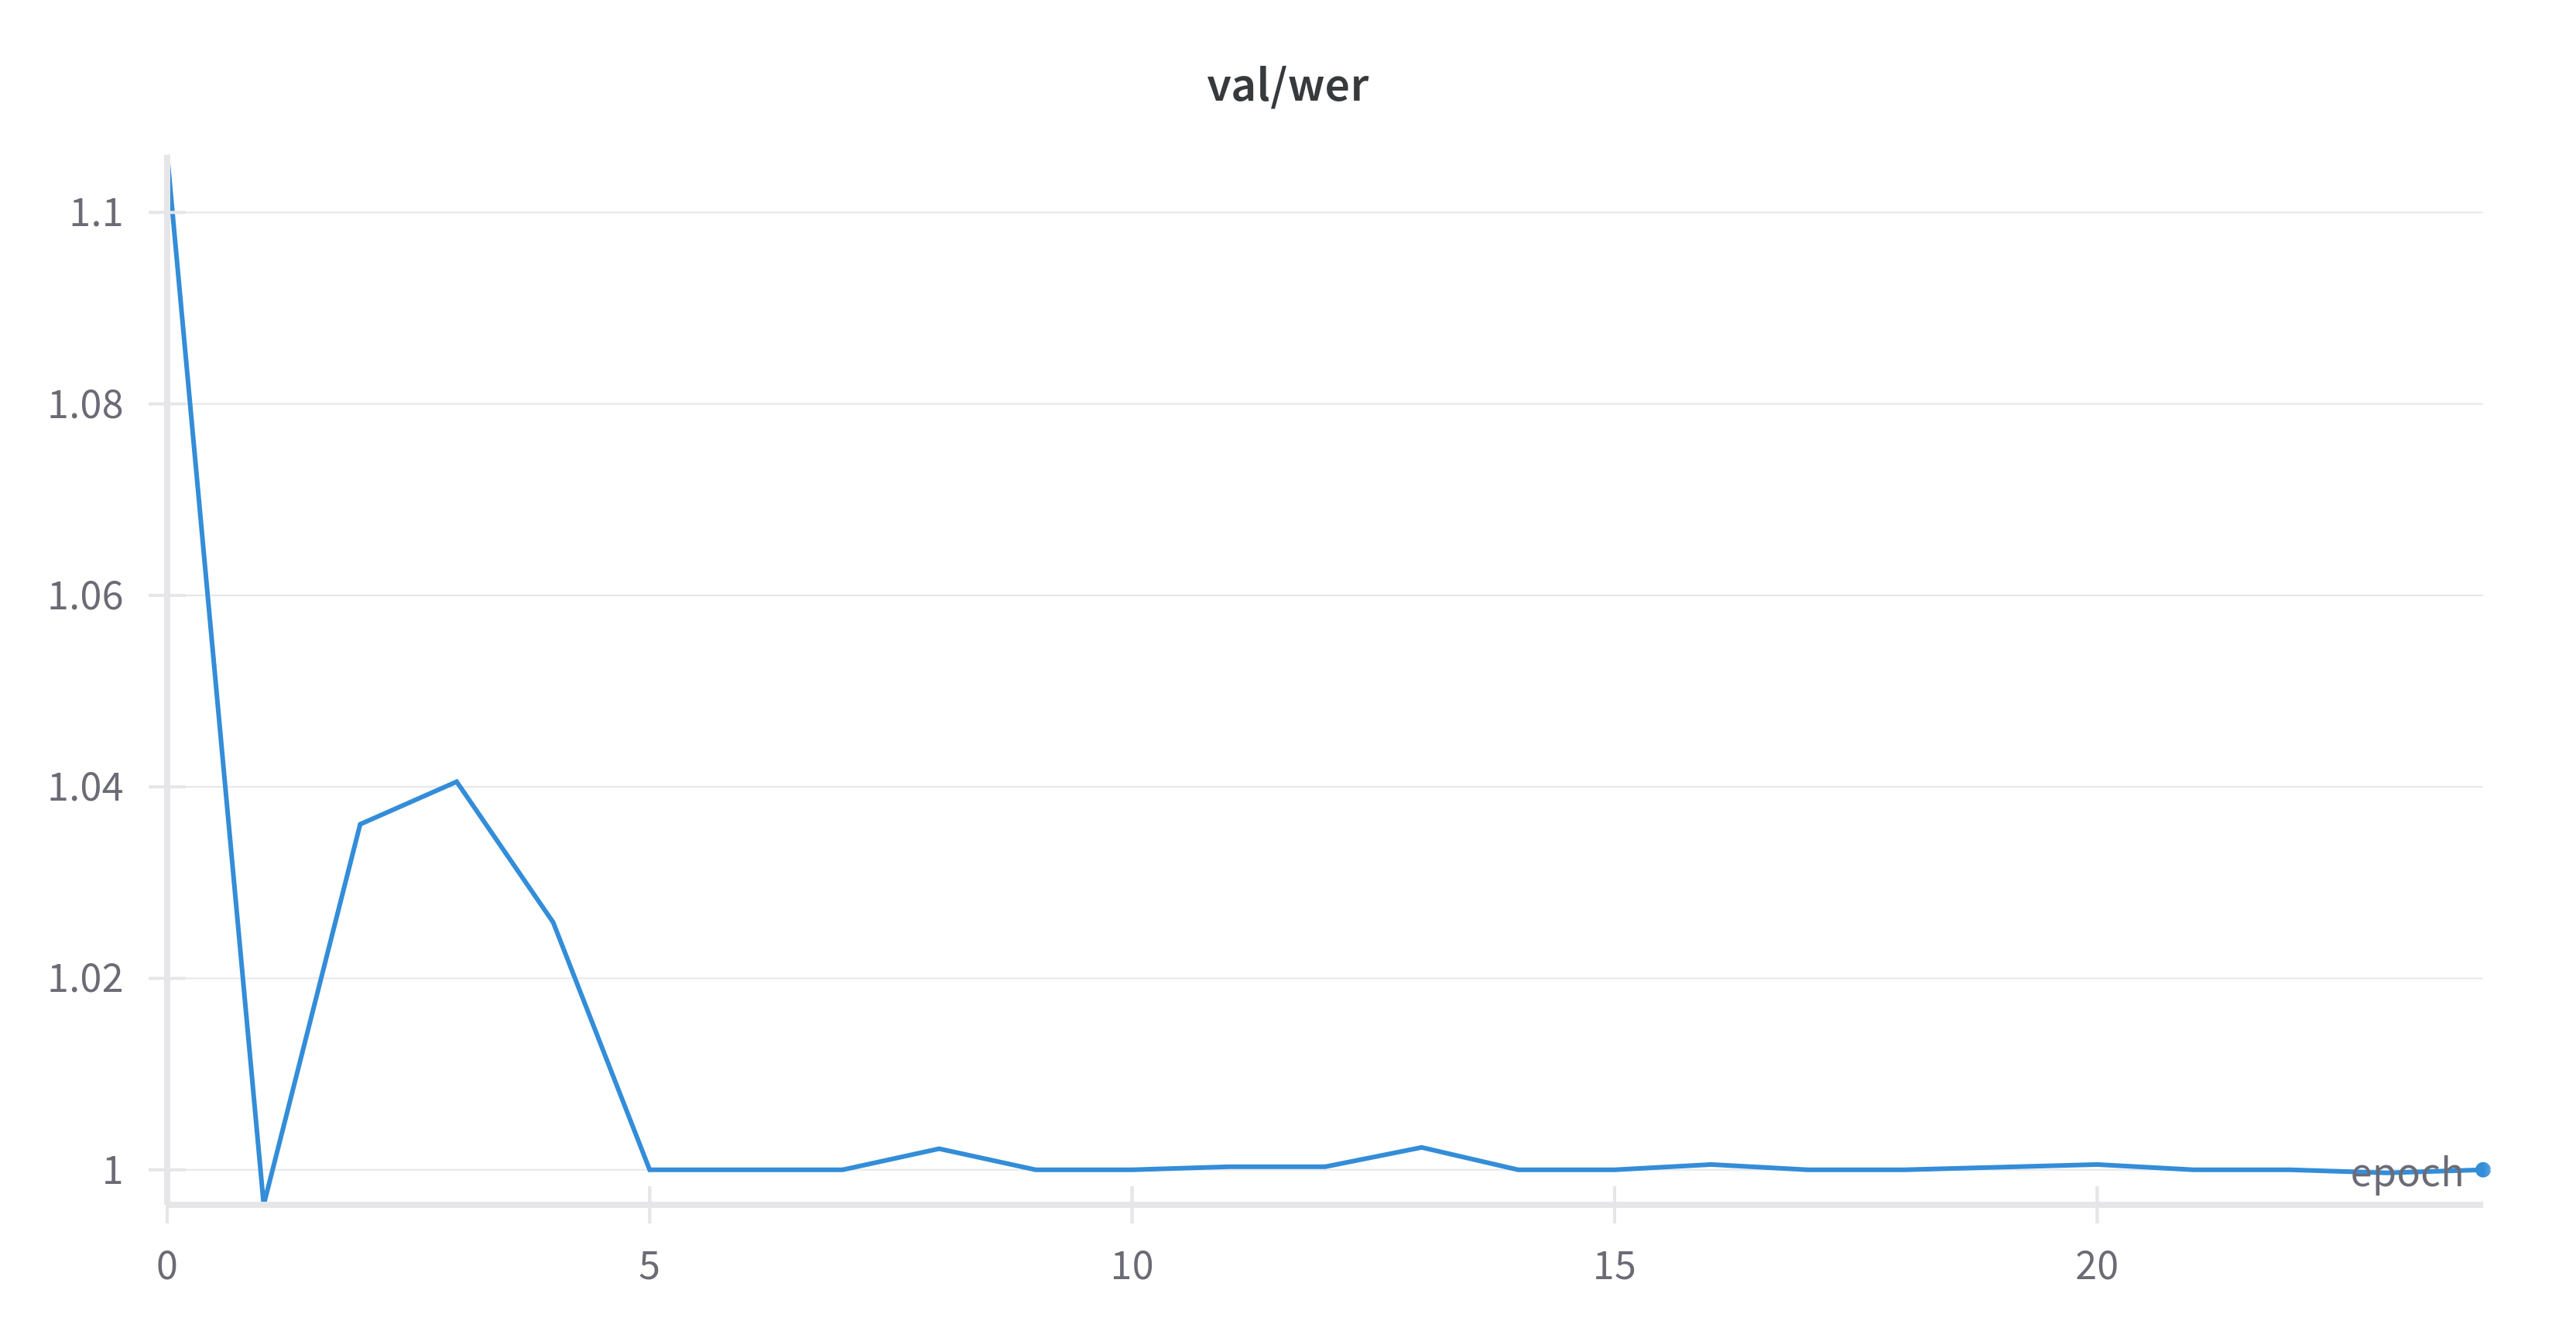
\includegraphics[width=1\textwidth]{figures/wer_ctc.png}
        \caption{Validation Word Error Rate for the encoder-only MobileViT, stuck at $1.0$.}
      \end{figure}
    \end{column}
  \end{columns}
\end{frame}


\begin{frame}
  \frametitle{Encoder Decoder MobileViT: Results}

  The encoder-decoder approach shows a \alert{smoother} convergence and a lower WER w.r.t. the encoder-only model.

  \begin{columns}
    \begin{column}{0.5\textwidth}
      \begin{figure}
        \centering
        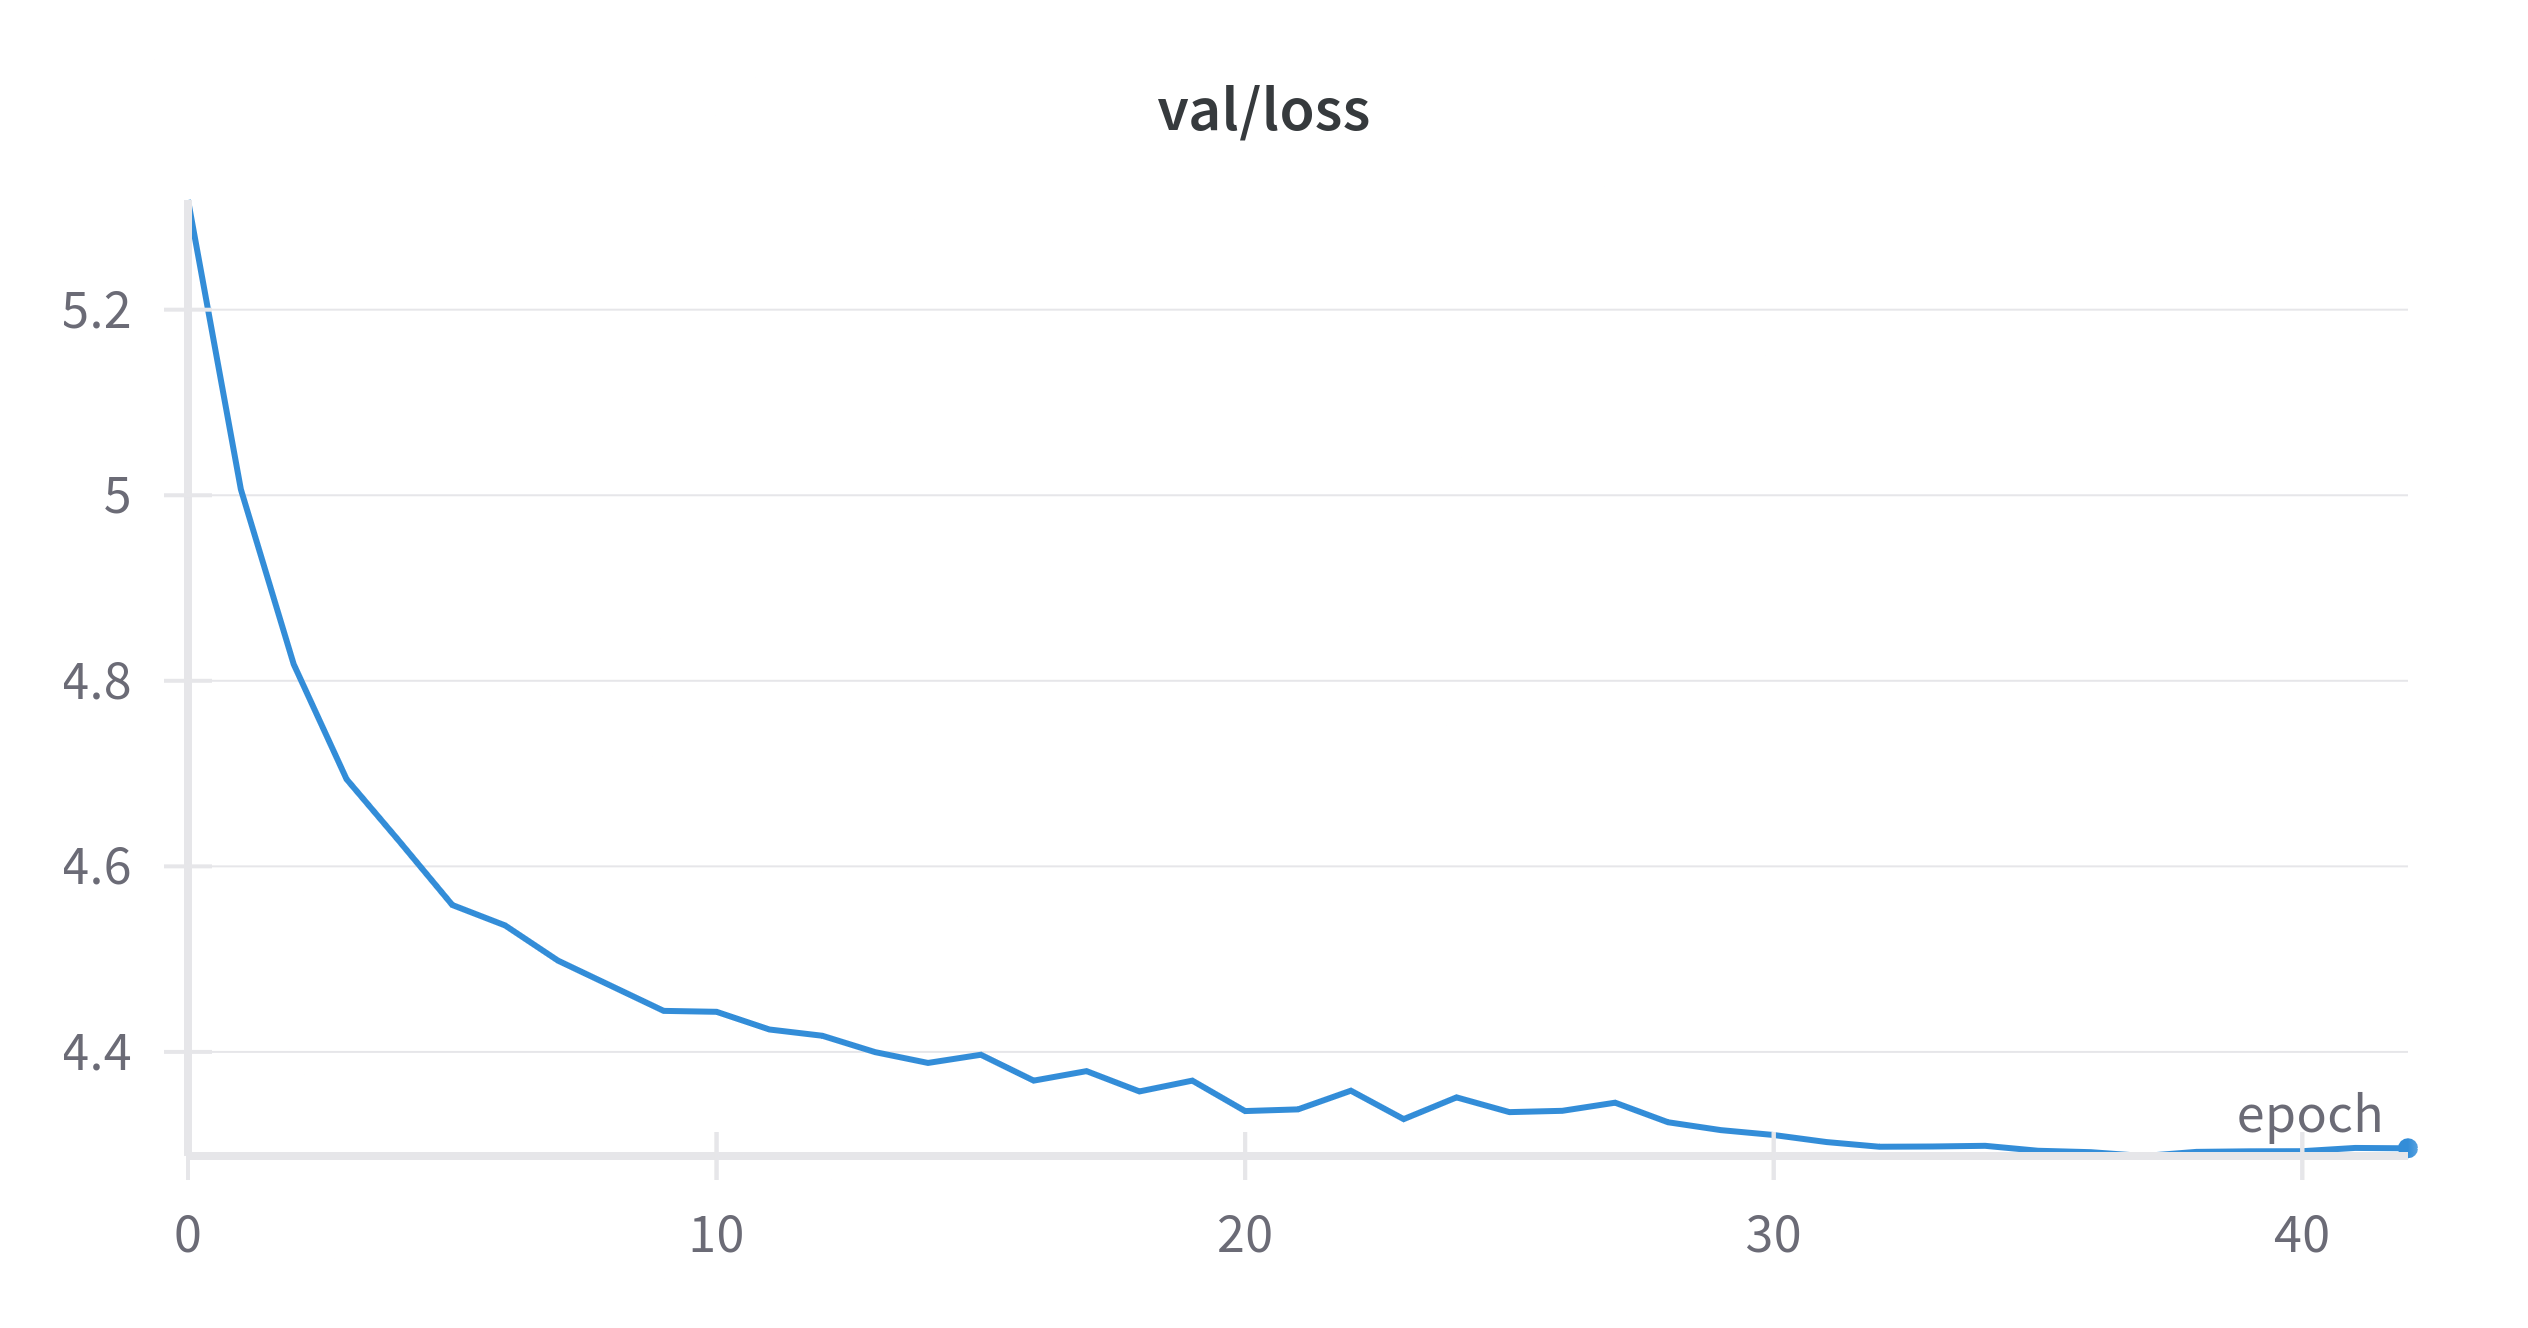
\includegraphics[width=1\textwidth]{figures/loss_encdec.png}
        \caption{Validation loss for the encoder-decoder MobileViT.}
      \end{figure}
    \end{column}
    \begin{column}{0.5\textwidth}
      \begin{figure}
        \centering
        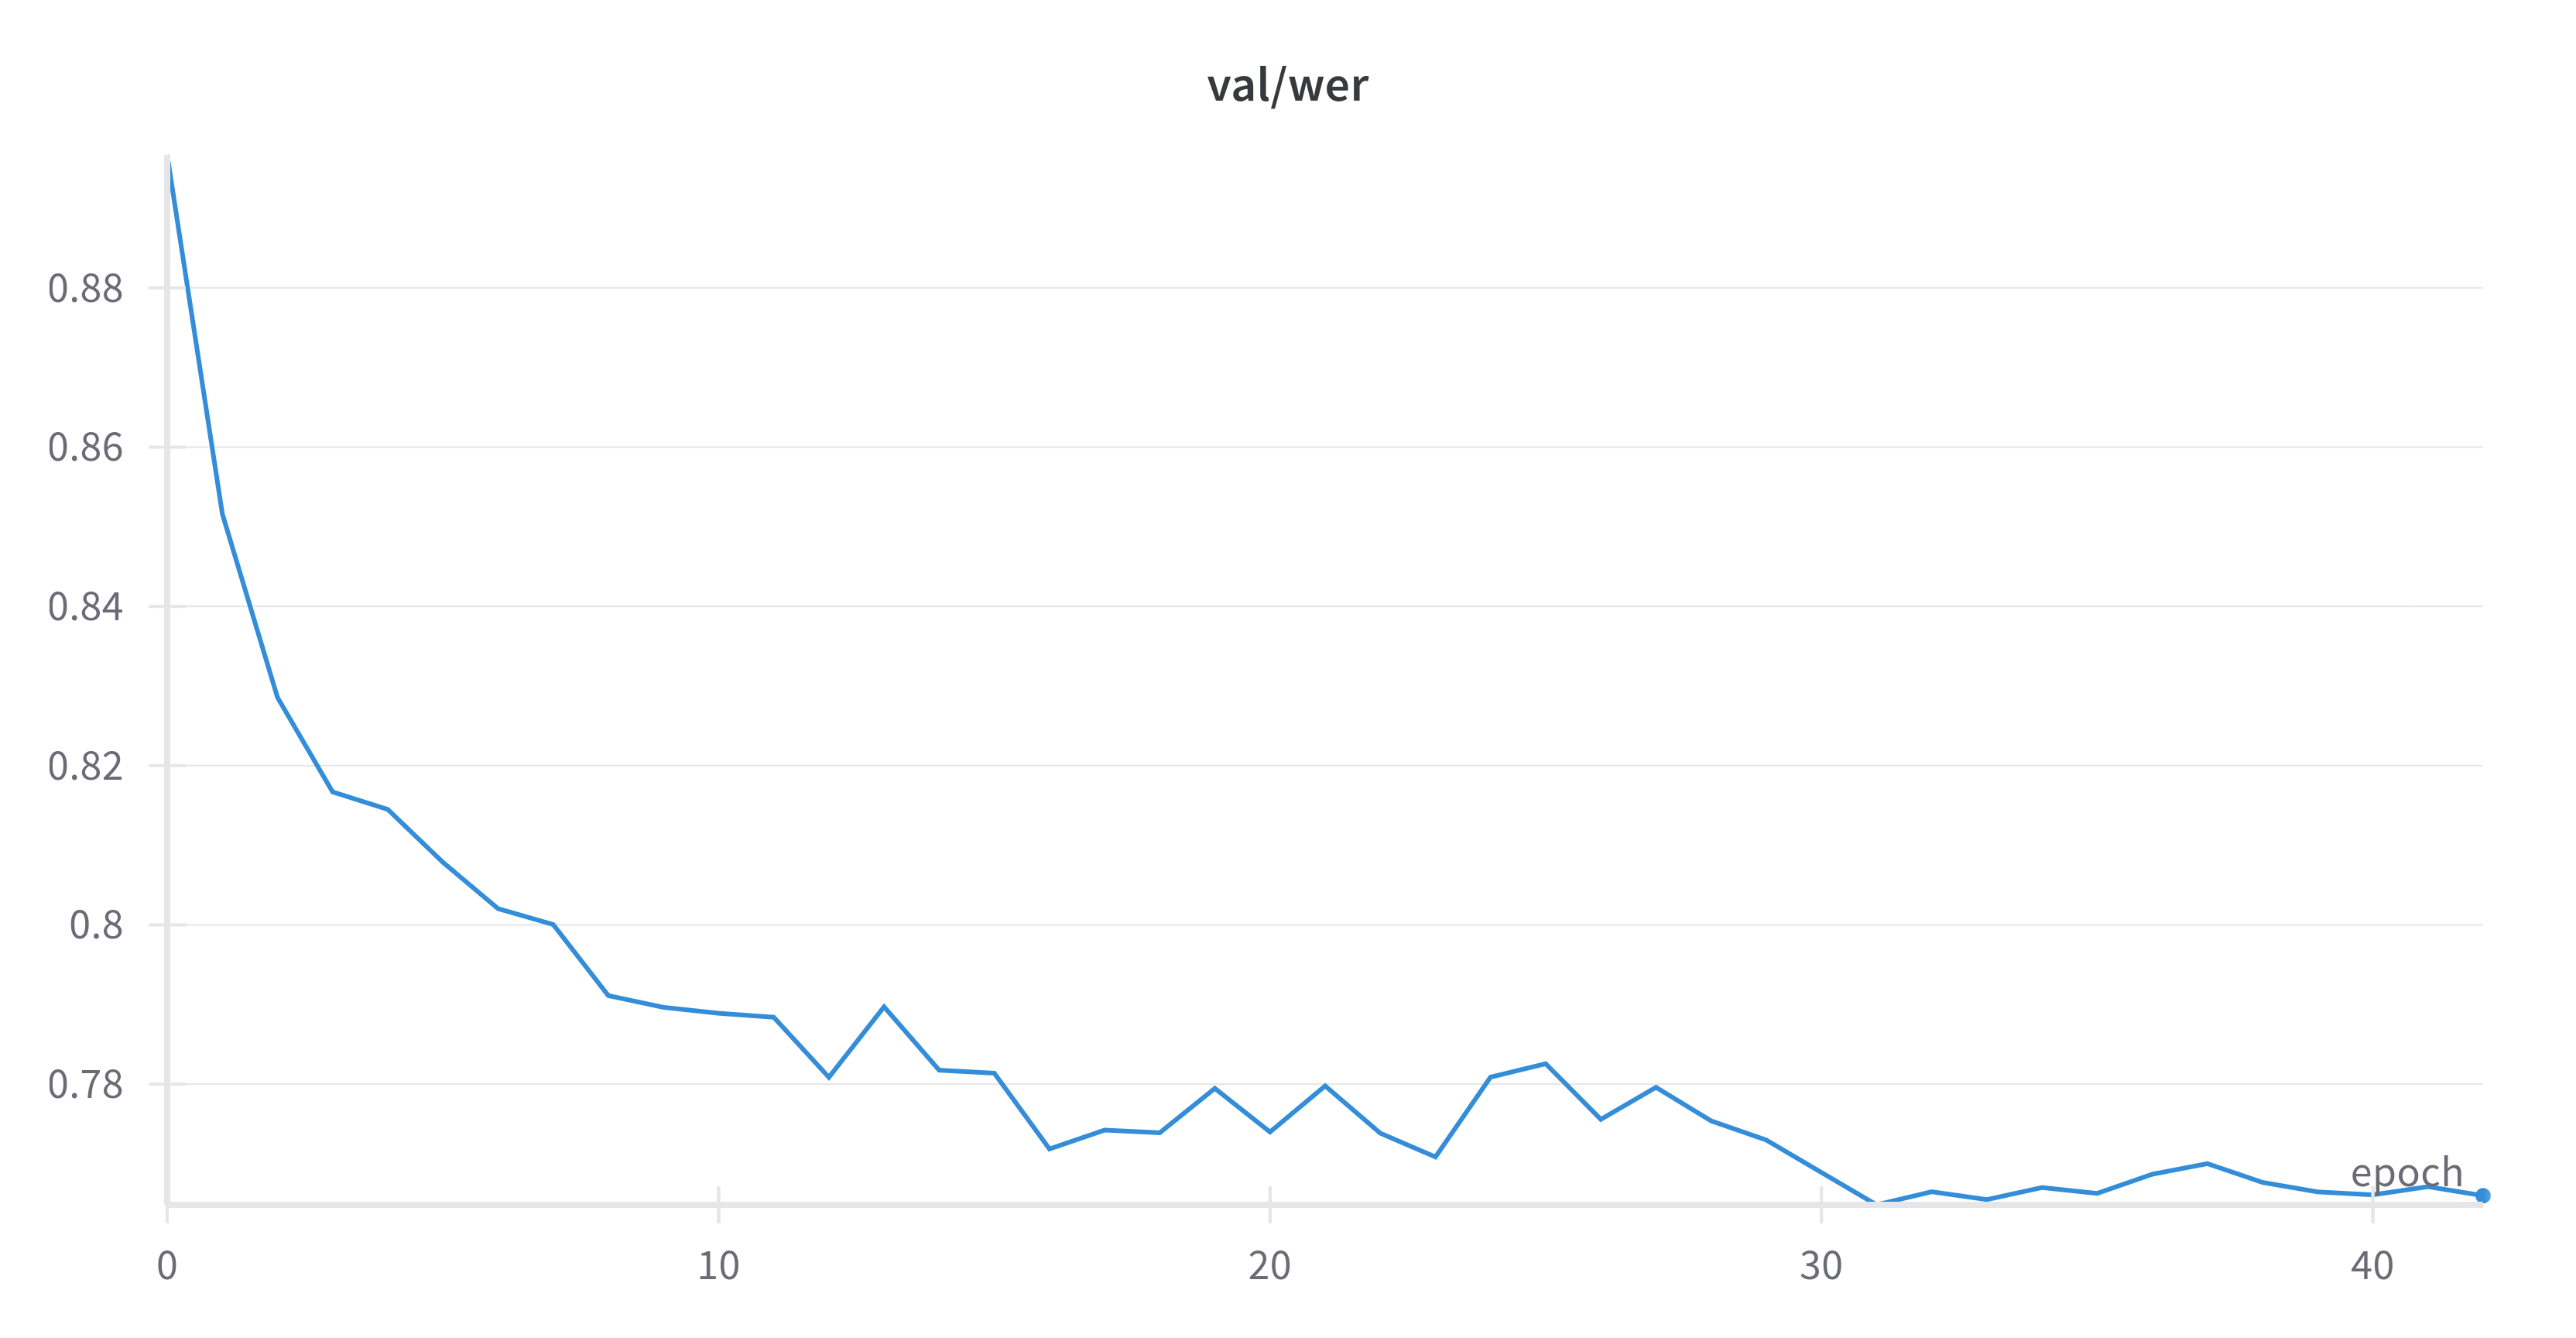
\includegraphics[width=1\textwidth]{figures/wer_encdec.png}
        \caption{Validation Word Error Rate for the encoder-decoder MobileViT.}
      \end{figure}
    \end{column}
  \end{columns}
\end{frame}

\begin{frame}
  \frametitle{Quantitative results}

  \begin{table}[H]
    \centering
    \begin{tabular}{lcc}
      \toprule
      \textbf{Model} & \textbf{Parameters (M)} & \textbf{WER} \\
      \midrule
      Encoder-only XXS MobileViT (ours) & 6.09 & 1.00 \\
      Encoder-decoder XXS MobileViT (ours) & 7.80 & 0.79 \\
      SlowFastSign\cite{ahn_slowfast_2023} & 52.90 & 0.18 \\
      LCSA\cite{zuo_local_2022} & 16.17 & 0.21 \\
      \bottomrule
    \end{tabular}
    \caption{Parameters (in millions) and validation Word-Error-Rate (WER) for the models.}
  \end{table}
\end{frame}

\section{Conclusions}

\begin{frame}
  \frametitle{Conclusions}

  CSLR is a challenging task that requires \alert{massive} computational resources. Even while employing
  models that are \alert{specifically} designed for mobile devices, we still struggle to achieve sufficient
  capacity to match state-of-the-art models.

  For both the encoder-only and encoder-decoder models, limited experiments with increasing parameter size
  showed \alert{improvements} in terms of WER. Showing that scaling the model up might be beneficial.
\end{frame}

\begin{frame}
  
  \centering
  \Huge
  \alert{Thank you for your attention!}
  
  \alert{Questions?}


\end{frame}

\section{Bibliography}

\bibliographystyle{abbrv}
\bibliography{ref}


\end{document}
